\chapter{Выполнение лабораторной работы}

\section{Цель работы}

Целью лабораторной работы №1 является освоение возможностей программы \texttt{Microsoft Project} для планирования проекта по разработке программного обеспечения.

\section{Тестовое задание}

 Осуществить планирование проекта с временными характеристиками, преставленными в таблице~\ref{tab:tz1}.
\begin{table}[H]
\caption{Временные характеристики тестового задания}
\label{tab:tz1}
\centering
\begin{tabular}{|c|c|}\hline
	Название работы & Длительность (дни) \\
	\hline
	Работа A & 12\\
	\hline
	Работа B & 6 \\
	\hline
	Работа C & 10\\
	\hline
	Работа D & 7\\\hline
	Работа E & 9\\\hline
	Работа F & 8\\\hline
	Работа G & 10\\\hline
	Работа H & 10\\\hline
	Работа I & 6\\\hline
	Работа J & 5\\\hline
\end{tabular}
\end{table}

Дата начала проекта~---~1-ый рабочий день марта текущего года. Провести планирование работ проекта, учитывая следующие связи между задачами:
\begin{itemize}
	\item предусмотреть, что C, J и D~---~исходные работы проекта, которые можно начинать одновременно;
	\item работа A следует за D, а работа I~---~за A;
	\item работа H следует за I;
	\item работа F следует за H, но не может начаться, пока не завершена C;
	\item работа G следует за I;
	\item работа E следует за J;
	\item работа B следует за E.
\end{itemize}

Дата начала проекта~---~2 марта 2026 года, что соответствует первому рабочему дню марта. Был создан список задач и установлены связи между задачами в соответствии с заданием. Результат представлен на рисунке \ref{fig:res1}.

\begin{figure}[H]
	\centering
	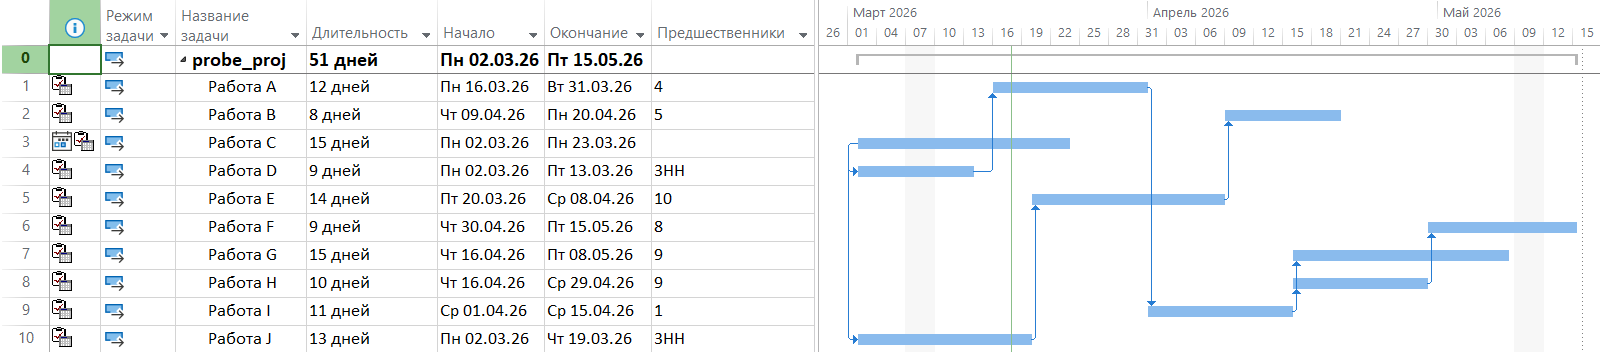
\includegraphics[width=\linewidth]{images/test_res_1.png}
	\caption{Список задач и диаграмма Ганта}
	\label{fig:res1}
\end{figure}

% \imgs{test-result}{h!}{0.3}{Результат выполнения тестового задания}


\section{Краткое описание проекта}

Команда разработчиков из 16 человек занимается созданием карты города на основе собственного модуля отображения. Проект должен быть завершен в течение 6 месяцев. Бюджет проекта: 50 000 рублей.

\section{Задание 1}

Настроить рабочую среду проекта:
\begin{enumerate}
	\item установить дату начала проекта~---~первый рабочий день марта текущего года;
	\item установить длительность работы в неделях, объем работ в часах, а тип работ по умолчанию~---~с фиксированными трудозатратами;
	\item установить количество рабочих часов в день равным 8, количество рабочих часов в неделю равным 40;
	\item задать начало рабочей недели в понедельник, а финансового года~---~в январе;
	\item установить продолжительность рабочего дня с 9 до 18 часов;
	\item установить стандартный календарь рабочего времени;
	\item отметить выходные и праздничные дни на ближайшие восемь календарных	месяцев от даты начала проекта;
	\item вывести на экран суммарную задачу проекта и заполнить вкладку <<Заметки>>	информацией об основных параметрах проекта.
\end{enumerate}

На рисунке~\ref{fig:sved} представлена вкладка <<Сведения о проекте>>, где установлена дата начала проекта и стандартный календарь, в котором отмечены сокращенные и праздничные дни.
\begin{figure}[H]
	\centering
	\includegraphics[width=\linewidth]{images/svedenia_o_projecte.png}
	\caption{Сведения о проекте}
	\label{fig:sved}
\end{figure}
	
На рисунке~\ref{fig:schedule} представлены сведения о длительности, объемах и типах работ, фиксированных трудозатратах, количестве рабочих часов в день и неделю, начале рабочей недели и финансового года.
%	\imgs{task1-2}{h!}{0.5}{Параметры проекта}
\begin{figure}[H]
	\centering
	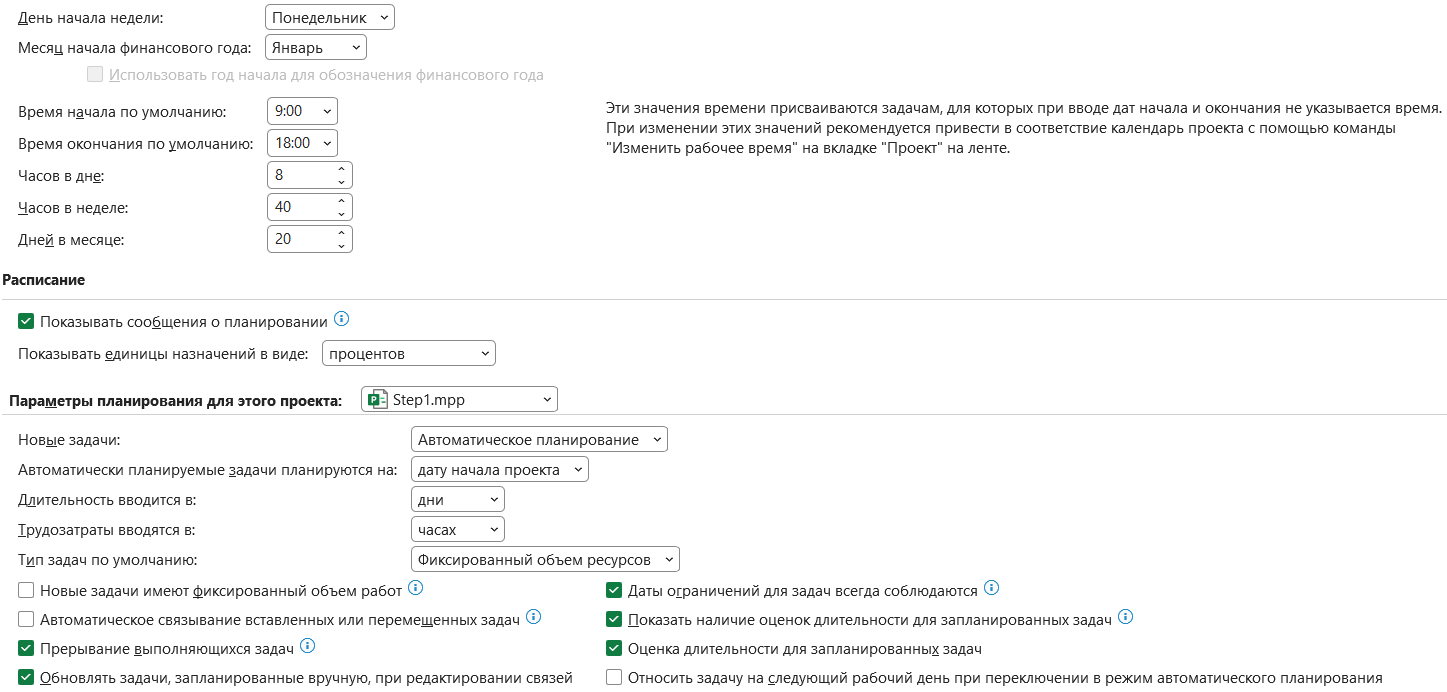
\includegraphics[width=0.9\linewidth]{images/schedule.png}
	\caption{Параметры расписания проекта}
	\label{fig:schedule}
\end{figure}

На рисунке~\ref{fig:notes} приведено содежание заметки к суммарной задаче.
%	\imgs{task1-4}{h!}{0.5}{Суммарная задача проекта и <<Заметки>>}
\begin{figure}[H]
	\centering
	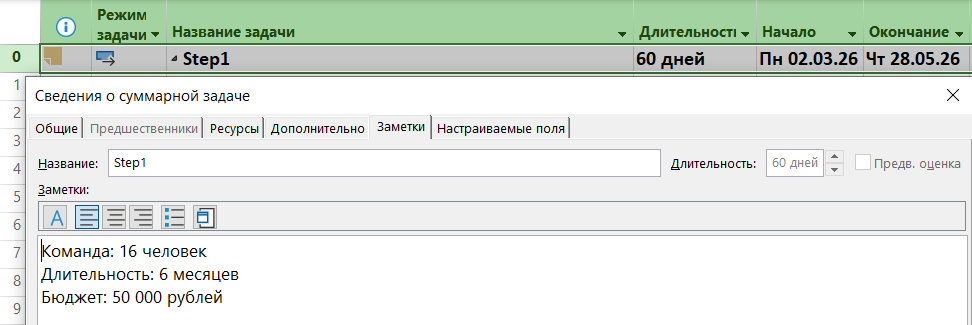
\includegraphics[width=\linewidth]{images/notes.png}
	\caption{Суммарная задача проекта и <<Заметки>>}
	\label{fig:notes}
\end{figure}

\section{Задание 2}

Создать список задач.

На рисунке~\ref{fig:step_1_res} приведен составленный список задач.
\begin{figure}[H]
	\centering
	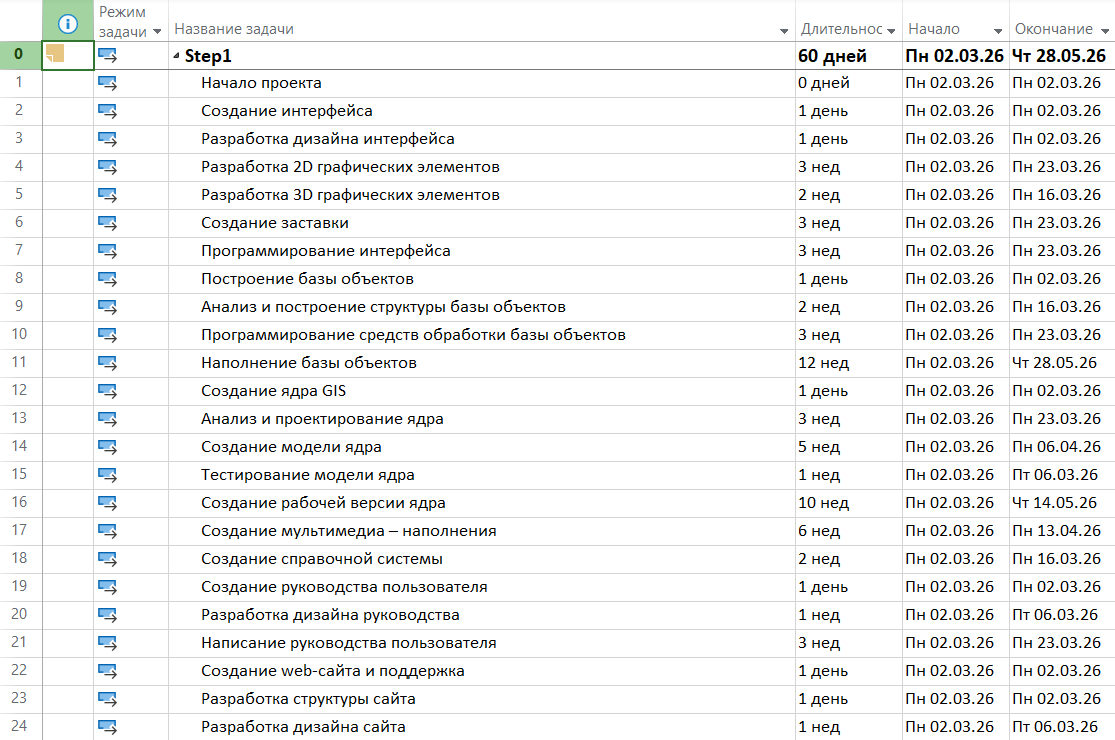
\includegraphics[width=\linewidth]{images/task_list.png}
	\caption{Список задач проекта}
	\label{fig:step_1_res}
\end{figure}
%\imgs{task2}{h!}{0.3}{Список задач}


\section{Задание 3}

Структурировать список задач проекта:
\begin{itemize}
	\item сгруппировать задачи 3--7 как подзадачи задачи 2;
	\item сгруппировать задачи 4--6 как подзадачи задачи 3;
	\item сгруппировать задачи 9--11 как подзадачи задачи 8;
	\item сгруппировать задачи 13--16 как подзадачи задачи 12;
	\item cгруппировать задачи 20, 21 как подзадачи задачи 19;
	\item сгруппировать задачи 23--25 как подзадачи задачи 22.
\end{itemize}

На рисунке~\ref{fig:groupped} приведен сгруппированный список задач проекта.

%\imgs{task3}{h!}{0.3}{Структура задач}

\begin{figure}[H]
	\centering
	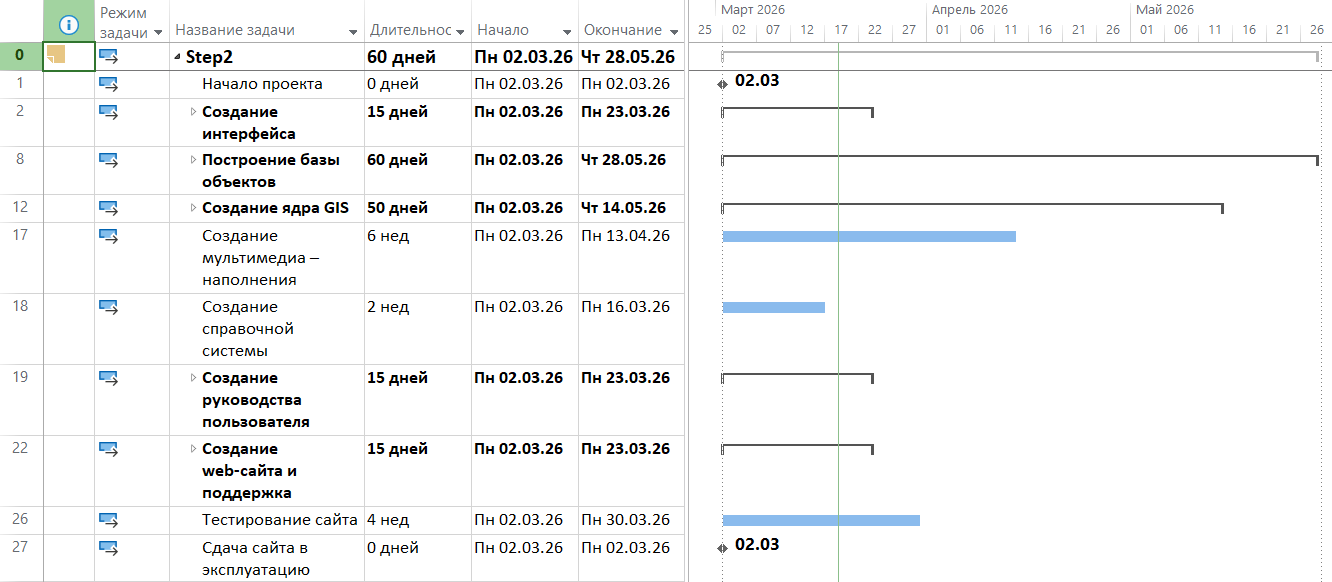
\includegraphics[width=\linewidth]{images/groupped_task_list.png}
	\caption{Группировка задач проекта}
	\label{fig:groupped}
\end{figure}


\section{Задание 4}

Установить связи между задачами проекта.

На рисунке~\ref{fig:linked} представлены связи между задачами проекта.

%\imgs{task4}{h!}{0.3}{Связи задач}

\begin{figure}[H]
	\centering
	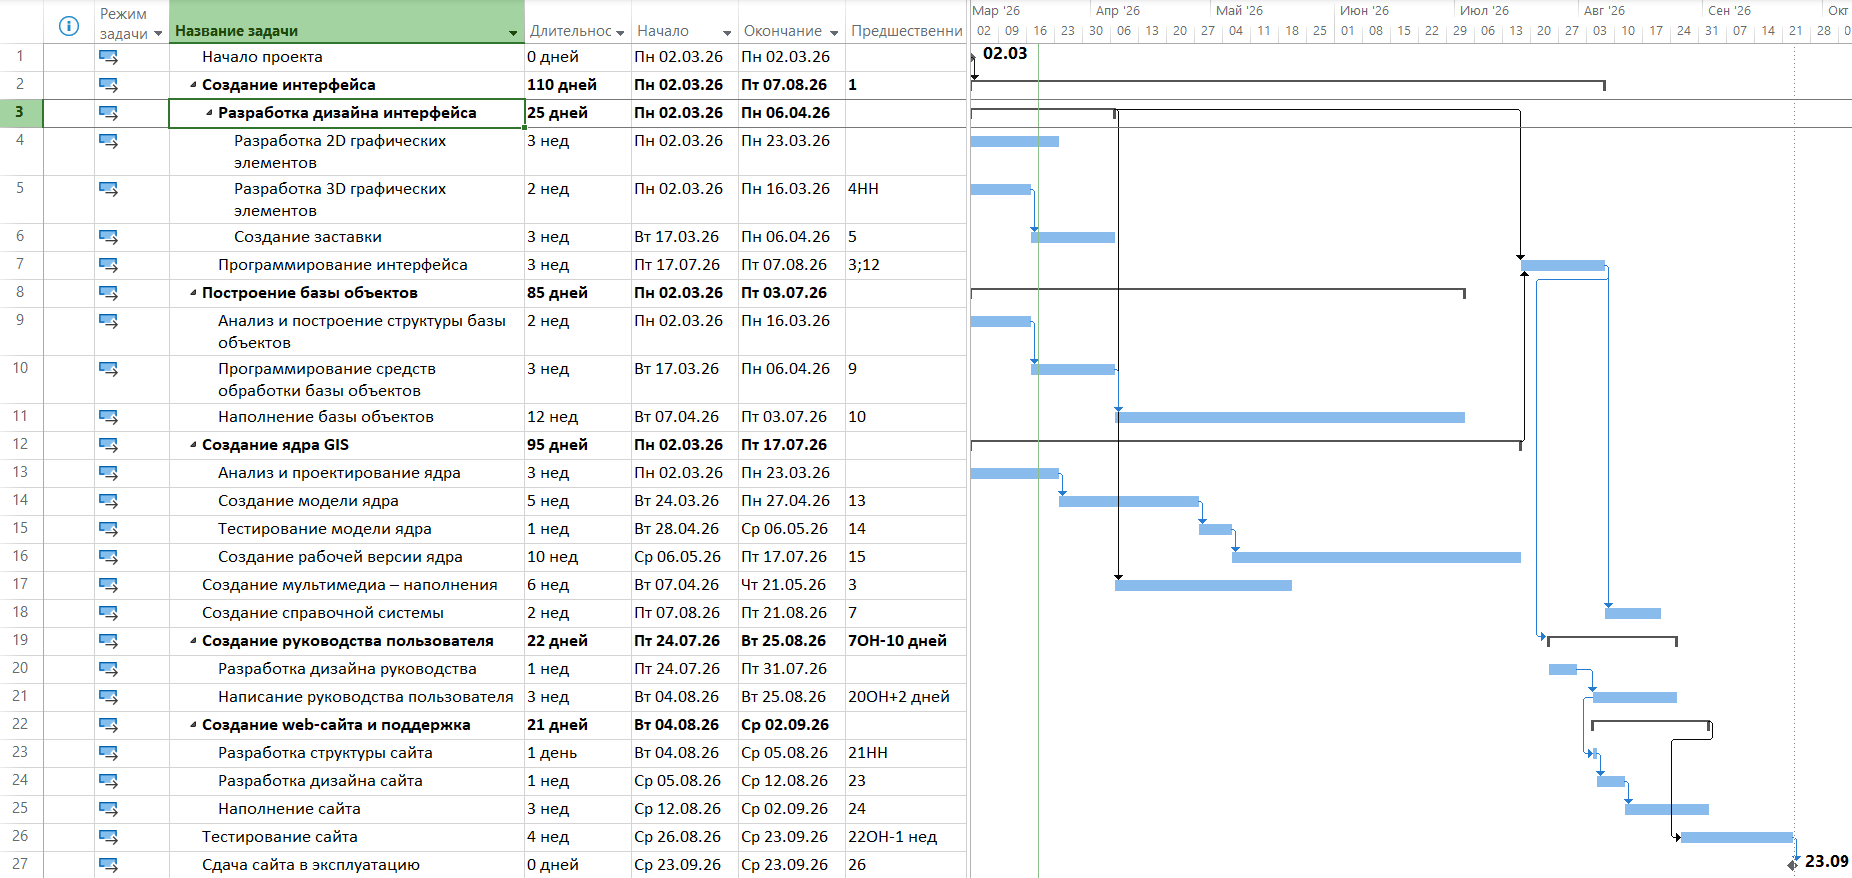
\includegraphics[width=\linewidth]{images/linked_task_list.png}
	\caption{Установленные связи между задачами}
	\label{fig:linked}
\end{figure}

\section*{Вывод}

В результате выполнения лабораторной работы было определено, что проект должен завершитья 23.09.23, что на 21 день больше ожидаемого срока выполнения проекта в 6 месяцев.